% Compile with XeLaTeX or LuaLaTeX for fontspec support
\documentclass{article}

\usepackage{arxiv}
\usepackage{fontspec}
\setmainfont{Linux Libertine O}
% \setmainfont{Inter}

\usepackage{polyglossia}
\setdefaultlanguage{english}
\setotherlanguage{russian}

\usepackage{url}
\usepackage{booktabs}
\usepackage{amsfonts, amssymb, amsmath, amsthm}
\usepackage{nicefrac}
\usepackage{microtype}
\usepackage{graphicx}
\usepackage{forest}

\usepackage{mathtools}
\usepackage{xcolor}
\usepackage{doi}
\usepackage{caption}

\usepackage[backend=biber, style=authoryear]{biblatex}
\addbibresource{references.bib}

\usepackage{ragged2e}
\usepackage{braket}
\usepackage[colorinlistoftodos]{todonotes}

\usepackage{booktabs}  % красивые линии
\usepackage{makecell}  % многострочные ячейки

% Custom TODO commands
\newcommand{\todoask}[1]{\todo[color=blue!30]{\textbf{Ask:} #1}}
\newcommand{\todocheck}[1]{\todo[color=green!30]{\textbf{Check:} #1}} 
\newcommand{\todoread}[1]{\todo[color=orange!30]{\textbf{Read:} #1}} 
\newcommand{\todocomment}[1]{\todo[color=purple!30]{\textbf{Comment:} #1}}

%% ============================================================================================================
%% Math commands and symbols
%% ============================================================================================================
\newcommand{\RMSE}[2]{\operatorname{RMSE}{\left(#1, #2\right)}}
\newcommand{\MAE}[2]{\operatorname{MAE}{\left(#1, #2\right)}}
\newcommand{\MAPE}[2]{\operatorname{MAPE}{\left(#1, #2\right)}}
\newcommand{\NSE}[2]{\operatorname{NSE}{\left(#1, #2\right)}}

\DeclareMathOperator*{\argmax}{arg\,max}
\DeclareMathOperator*{\argmin}{arg\,min}

\newcommand{\Indicator}[1]{\mathbf{1}_{\set{#1}}}
\newcommand{\SetPower}[1]{\##1}

\newcommand{\Reals}{\mathbb{R}}

\newcommand{\Ell}{\mathcal{L}}
\newcommand{\Dataset}{\mathcal{D}}
\newcommand{\Models}{\mathcal{F}}
\newcommand{\Model}{\hat{f}}
\newcommand{\BestModel}{f^*}


%% ============================================================================================================
%% Metadata
%% ============================================================================================================
\title{Untangling Equifinality: A Large-Sample Benchmark of Machine-Learning Models for Rainfall–Runoff Forecasting in Eurasian Basins}

\author{
    Khuzin Eldar \\
    Chair of Data Analysis\\
    Moscow Institute of Physics and Technology\\
    Moscow, Russia \\
    \texttt{khuzin.er@phystech.su} \\
    \And
    Novikov Ivan \\
    Affiliation \\
    Address \\
    \texttt{email} \\
    \And
    Abramov Dmitrii \\
    Affiliation \\
    Address \\
    \texttt{email}
}

\date{}

\hypersetup{
    pdftitle={Comparative Analysis of Data-Driven Approaches for Hydrological Forecasting},
    pdfsubject={cs.LG},
    pdfauthor={Eldar Khuzin, Novikov Ivan, Abramov Dmitrii},
    pdfkeywords={Flood discharge, Rainfall-runoff modeling, More}
}

%% ============================================================================================================
%% Document begin
%% ============================================================================================================
\begin{document}
\sloppy
\justifying

\maketitle

%% ============================================================================================================
%% Abstract
%% ============================================================================================================

\begin{abstract}
    In this article, we address the problem of equifinality in data-driven hydrological modeling. Equifinality is when different feature sets or model architectures yield similar predictive efficiency. We investigate the influence of static catchment features on predictions made by traditional machine learing models(e.g., random forest, gradient boosting), recurrent neural networks \todo{and transformers} across various river basins in Eurasia. By analyzing feature importance and model behavior, we identify dominant predictors and assess the practicality of employing complex models in terms of interpretability and computational cost. This approach provides insights into the trade-offs between model complexity and predictive robustness in the presence of equifinality.
\end{abstract}


\keywords{
    Flood discharge
    \and Rainfall–Runoff Modeling
    \and Equifinality
    \and Machine Learning
    \and SHAP
    \and Static Catchment Characteristics
}


\listoftodos[List of suggested changes]

\begin{table}[htbp]
    \centering
    % ширину текстовых столбцов удобно задать явно,
    % чтобы переносы строк не «выпирали»
    \begin{tabular}{c p{3.2cm} p{4.0cm} p{4.0cm}}
        \toprule
        \textbf{cluster} & \textbf{rank 1} & \textbf{rank 2} & \textbf{rank 3} \\
        \midrule
        0                &
        \makecell[l]{lat\_z                                                    \\Широта} &
        \makecell[l]{for\_pc\_sse\_z                                           \\Площадь лесного покрова, \%} &
        \makecell[l]{gwt\_cm\_sav\_z                                           \\Глубина уровня грунтовых вод, см}\\[2pt]

        1                &
        \makecell[l]{crp\_pc\_sse\_z                                           \\Площадь пахотных земель, \%} &
        \makecell[l]{for\_pc\_sse\_z                                           \\Площадь лесного покрова, \%} &
        \makecell[l]{pst\_pc\_sse\_z                                           \\Площадь пастбищ, \%}\\[2pt]

        2                &
        \makecell[l]{cly\_pc\_sav\_z                                           \\Доля глины в почве, \%} &
        \makecell[l]{slt\_pc\_sav\_z                                           \\Доля ила в почве, \%} &
        \makecell[l]{snd\_pc\_sav\_z                                           \\Доля песка в почве, \%}\\[2pt]

        3                &
        \makecell[l]{inu\_pc\_ult\_z                                           \\Площадь затопления, \%} &
        \makecell[l]{lka\_pc\_use\_z                                           \\Доля площади озёр, \%} &
        \makecell[l]{lat\_z                                                    \\Широта}\\[2pt]

        4                &
        \makecell[l]{sgr\_dk\_sav\_z                                           \\Градиент русла} &
        \makecell[l]{gwt\_cm\_sav\_z                                           \\Глубина уровня грунтовых вод, см} &
        \makecell[l]{slp\_dg\_sav\_z                                           \\Уклон поверхности, $^\circ$}\\[2pt]

        5                &
        \makecell[l]{lon\_z                                                    \\Долгота} &
        \makecell[l]{lat\_z                                                    \\Широта} &
        \makecell[l]{slp\_dg\_sav\_z                                           \\Уклон поверхности, $^\circ$}\\[2pt]

        6                &
        \makecell[l]{prm\_pc\_sse\_z                                           \\Площадь вечной мерзлоты, \%} &
        \makecell[l]{lon\_z                                                    \\Долгота} &
        \makecell[l]{ws\_area\_z                                               \\Площадь водосбора, км$^{2}$}\\[2pt]

        7                &
        \makecell[l]{ele\_mt\_sav\_z                                           \\Высота над ур.\ моря, м} &
        \makecell[l]{height\_bs\_z                                             \\Средняя высота бассейна, м} &
        \makecell[l]{prm\_pc\_sse\_z                                           \\Площадь вечной мерзлоты, \%}\\[2pt]

        8                &
        \makecell[l]{lkv\_mc\_usu\_z                                           \\Объём озёр, млн м$^{3}$} &
        \makecell[l]{cly\_pc\_sav\_z                                           \\Доля глины в почве, \%} &
        \makecell[l]{slt\_pc\_sav\_z                                           \\Доля ила в почве, \%}\\
        \bottomrule
    \end{tabular}
    \caption{Кластеры и три наиболее информативных признака (с русскими определениями).}
    \label{tab:cluster_ranks_ru}
\end{table}

%% ============================================================================================================
%% Introduction
%% ============================================================================================================
%% ============================================================================================================
%% Introduction
%% ============================================================================================================
\section{Introduction}
\label{sec:introduction}

Accurate rainfall--runoff forecasting is essential for water--resource management (long--term water--resource planning, reservoir operation) and flood risk assessment. Nevertheless, forecast skill in the calibration period does not automatically translate into reliable predictions for unseen basins or extreme events; rigorous tests of model generalisation are therefore indispensable.

Traditionally, physically based hydrological models are calibrated separately for each basin; yet it is often observed  that markedly different parameter sets or model structures can reproduce the same hydrograph with near--identical accuracy --- a phenomenon known as \emph{equifinality} (literally ``equal finality'') \cite{bevenFutureDistributedModels1992a, freerBayesianEstimationUncertainty1996}. Equifinality undermines the notion of a unique ``best'' model and complicates any attempt to ascribe physical meaning to fitted parameters.

Machine--learning (ML) methods intensify this challenge. The flexibility of modern data--driven methods --- from tree ensembles to deep neural networks --- gives them many ``degrees of freedom'' to fit data and can exploit subtle correlations that lack causal significance. High predictive skill alone therefore \emph{does not guarantee} that an ML model has learned the underlying hydrological processes. When several equifinal models agree on historical data, some may break down under non-stationary climate or in ungauged basins.

Static catchment descriptors --- such as drainage area, mean slope, soil texture, and aridity index--offer a partial remedy by injecting physical context into data--driven models; incorporating them into an LSTM has been shown to yield a ``universal'' regional model that generalises across basins \cite{kratzertLearningUniversalRegional2019}. Yet under equifinality different architectures may leverage the same descriptors in different ways or ignore them altogether while still achieving comparable accuracy. Determining which inputs truly drive predictions is thus a prerequisite for trustworthy operational use.

This study disentangles equifinality in data--driven rainfall--runoff modeling through a controlled, large-sample comparison of three representative ML architectures: a random forest, a gradient boosting and a long short--term memory (LSTM) network. All models receive identical meteorological time series and static basin attributes, eliminating data inequality as a confounder. We evaluate their predictive skill --- quantified by Nash--Sutcliffe efficiency (NSE), root mean square error (RMSE), and mean absolute percentage error (MAPE) --- on 1,073 Eurasian basins and inspect feature contributions via SHAP values.

Our contributions are three--fold:
\begin{enumerate}
    \item We quantify how often alternative architectures yield statistically indistinguishable performance, providing a basin--wise map of equifinality.
    \item We reveal the degree to which equifinal models rely on the same (or different) static and dynamic predictors.
    \item We discuss the trade--off between accuracy, interpretability, and computational cost, offering guidance for practitioners choosing between simple and complex ML tools.
\end{enumerate}

The remainder of the paper is organised as follows. Section~\ref{sec:data} describes the data set and study area. Section~\ref{sec:methods} details the models, training procedure, loss functions, and evaluation metrics. Section~\ref{sec:computational-experiment} describes the experiments. Section~\ref{sec:results} presents the experimental results, including an analysis of equifinality and feature importance. Section~\ref{sec:discussion} discusses the implications for hydrological theory and operational forecasting. Finally, Section~\ref{sec:conclusion} summarises the key findings and outlines future work.

\todo[inline]{Написать о выделение кластеров и внутри кластеров исследуем эквифинальность модели "выделение различных статических атрибутов" --- квазиосознаность.}


%% ============================================================================================================
%% Data and Study Area
%% ============================================================================================================
%% ============================================================================================================
%% Data and Study Area
%% ============================================================================================================
\section{Data and Study Area}
\label{sec:data}

% Study Area
% ————————————————————————————————————————————————————————————————————————————
\subsection{Study Area}

This study focuses on river basins across Eurasia, located approximately between latitudes \todo{latitudes} and longitudes \todo{longitudes}. The selected region encompasses a wide range of static basin characteristics and climatic conditions, making it suitable for analyzing hydrological equifinality.

\todo[inline]{Add a map of the river basins}

% Hydrometeorological Data
% ————————————————————————————————————————————————————————————————————————————
\subsection{Hydrometeorological Data}

The dataset includes daily time series from 2008 to 2022 for the following features:
precipitation (\texttt{prcp}), river water level (\texttt{lvl\_sm}), minimum temperature (\texttt{t\_min}), maximum temperature (\texttt{t\_max}), mean temperature (\texttt{t\_mean} \todo{check the name of t\_mean}), and river discharge (\texttt{q\_mm\_day}).

\todo[inline]{Add an example time series plot.}

% Static Basin Attributes
% ————————————————————————————————————————————————————————————————————————————
\subsection{Static Basin Attributes}

Static (time-invariant) characteristics of the river basins were derived from the HydroSHEDS database \todo{Add cite to https://www.hydrosheds.org/}. A total of 12 features\ref{table:static-attributes} were selected based on two main criteria: (i) low pairwise correlation and (ii) high interpretability for ability to explain the models.

In total, data were available for 2,201 river basins. For model training and subsequent analysis, we selected a subset of 1,073 basins with the fewest missing values to ensure data quality and consistency across samples.

\begin{table}[ht]
    \centering
    \begin{tabular}{lll}
        \toprule
        \textbf{ID}  & \textbf{Attribute}              & \textbf{Column Name}  \\
        \midrule
        \textbf{L07} & Forest Cover Extent             & \texttt{for\_pc\_sse} \\
        \textbf{L08} & Cropland Extent                 & \texttt{crp\_pc\_sse} \\
        \textbf{L09} & Pasture Extent                  & \texttt{pst\_pc\_sse} \\
        \textbf{L10} & Irrigated Area Extent           & \texttt{ire\_pc\_sse} \\
        \textbf{A03} & Urban Extent                    & \texttt{urb\_pc\_sse} \\
        \textbf{S07} & Karst Area Extent               & \texttt{kar\_pc\_sse} \\
        \textbf{P01} & Elevation                       & \texttt{ele\_mt\_sav} \\
        \textbf{P02} & Terrain Slope                   & \texttt{slp\_dg\_sav} \\
        \textbf{C06} & Aridity Index                   & \texttt{ari\_ix\_sav} \\
        \textbf{H10} & Groundwater Table Depth         & \texttt{gwt\_cm\_sav} \\
        \textbf{S05} & Soil Water Content (Annual Avg) & \texttt{swc\_pc\_syr} \\
        \textbf{S01} & Clay Fraction in Soil           & \texttt{cly\_pc\_sav} \\
        \textbf{A06} & Human Footprint Index           & \texttt{hft\_ix\_s09} \\
        \textbf{P04} & Latitude                        & \texttt{lat}          \\
        \textbf{P05} & Longitude                       & \texttt{lon}          \\
        \bottomrule
    \end{tabular}
    \caption{List of selected static features and their corresponding column names.}
    \label{table:static-attributes}
\end{table}



%% ============================================================================================================
%% Methods
%% ============================================================================================================
%% ============================================================================================================
%% Methods
%% ============================================================================================================
\section{Methods}
\label{sec:methods}

\todo[inline]{Общий pipeline}

% Problem statement and notation
% ————————————————————————————————————————————————————————————————————————————
\subsection{Problem Statement and Notation}

We address a regression problem where we aim to predict a target from a set of features.

\paragraph{Notation}
\begin{itemize}
    \item Let \(y \in \Reals^n\) and \( y_i \in \Reals \) denote the target; \(x \in \Reals^{n \times d}\) and \( x_i \in \Reals^d \) denote \(d\) features associated with \( y_i \), where \(n\) is the number of samples;
    \item Let the dataset be \( \Dataset = \set{(x_i, y_i) \mid i \in \overline{1, n}} \) --- set of \(n\) pairs for features and targets.
    \item Let the models class be denoted as \(\Models\);
    \item Let \( \hat{y}_i \coloneqq f(x_i),\, f \in \Models\) denotes estimation of \( y_i \) based on \( x_i \);
    \item Let assume \(\hat{y} \coloneqq \left( \hat{y}_1, \dots, \hat{y}_n \right) = \left( f(x_1), \dots, f(x_n) \right)\).
\end{itemize}
% ————————————————————————————————————————————————————————————————————————————
% End of 'Problem statement and notation'

% Optimization statement
% ————————————————————————————————————————————————————————————————————————————
\subsection{Optimization statement}

In general, in each experiment we find the optimal model \(\BestModel\) s.t.

\begin{equation}
    \BestModel
    =
    \argmin\limits_{f \in \Models}{\left( \Ell(f, \Dataset) + \Omega(f) \right)},
    \label{oprimization:general-task}
\end{equation}

where \( \Ell(f, \Dataset) \) denotes the empirical loss of model \(f\) on dataset \(\Dataset\), and \( \Omega(f) \) is a regularization term penalizing model complexity.

Let \(\ell(\cdot, \cdot)\) denotes the actual loss function, so \(\Ell(f, \Dataset) = \ell(y, \hat{y}) = \frac{1}{n}{\sum\limits_{i=1}^{n}{\ell(y_i, \hat{y}_i)}} \).

In our work we choose\todo{Link to article and explanation why MAPE} \(\ell\) as a mean absolute percentage error (\ref{metric:mape}), so \ref{oprimization:general-task} can be rewriten as

\begin{equation}
    \BestModel
    =
    \argmin\limits_{
        f \in \Models
    }{
        \left(
        \sum_{i=1}^{n} \left| \frac{y_i - f({x_i})}{y_i} \right| + \Omega(f)
        \right)
    }.
    \label{oprimization:task}
    \tag{Opt.~task}
\end{equation}

\subsubsection{Pseudo-MAPE Objective}

But standard \ref{metric:mape} is non-differentiable at \(y_i=\hat y_i\) and yields unbounded gradients as \( y_i \to 0\).
To obtain smoother, more stable updates in gradient-based learners, we define a pseudo-MAPE loss with smoothing parameter \(\delta>0\):
\[
    L_\delta(r)
    = \sqrt{r^2 + \delta^2},\quad
    r_i = \frac{\hat y_i - y_i}{y_i}\,.
\]
Its gradient and Hessian (needed for XGBoost’s custom objective) are
\[
    g_i = \frac{r_i}{y_i\,\sqrt{r_i^2 + \delta^2}},\quad
    h_i = \frac{\delta^2}{y_i^2\,\bigl(r_i^2 + \delta^2\bigr)^{3/2}}.
\]
In our experiments we set \(\delta=10^{-1}\) to balance smoothness and closeness to true MAPE.

\todo[inline]{pseudo-MAPE vs MAPE plot}

% ————————————————————————————————————————————————————————————————————————————
% End of 'Optimization statement'

% Model's description
% ————————————————————————————————————————————————————————————————————————————
\subsection{Model's descriptions}

% Regression trees
% ------------------------------------------------------
\subsubsection{Regression trees}\todo{Add link to article, where trees were presented}
\label{model:regression-tree}

In experiments we use regression trees as base predictors. In general, regression tree is binary tree, which partitions the feature space into regions and predicts constant values within each region, formally:
\begin{equation}
    f(x)
    =
    \sum\limits_{l=1}^{L}\Indicator{x \in R_l}\cdot\omega_l,
\end{equation}
where:
\begin{itemize}
    \item \(R_l,\, l \in \overline{1, L}\) form a partition of \(\Reals^d\) into disjoint sets;
    \item \(\omega_l\) are constant weights on tree leaves.
\end{itemize}

To perform the partitioning into \( R_l \), each node of the binary tree acts as a simple predicate of the form \( x^{(j)} \le t \), used to select between the left and right child. Here, \( x^{(j)} \) denotes a coordinate in the features \( \Reals^d \) space, and \( t \) is a \emph{threshold}.

\todo[inline]{Add a picture of three}

To select a threshold \( t \) and the corresponding feature index \( j \) at each node, the algorithm maximizes an objective function known as the \emph{information gain (IG, \(\mathcal{IG}\))}. We are going to use the same IG as \cite{chenXGBoostScalableTree2016a}. Let assume \(\hat{y}_i^{(0)}\) as initial prediction (constant)\todo{Think about initial value.}:
\[
    \mathcal{IG}(t, j)
    =
    \frac{1}{2}
    \left[
        \frac{\left(\sum_{i\in \mathcal{I}_L} g_i\right)^2}{\sum_{i\in \mathcal{I}_L} h_i + \lambda}
        +
        \frac{\left(\sum_{i\in \mathcal{I}_R} g_i\right)^2}{\sum_{i\in \mathcal{I}_R} h_i + \lambda}
        -
        \frac{\left(\sum_{i\in \mathcal{I}} g_i\right)^2}{\sum_{i\in \mathcal{I}} h_i + \lambda}
        \right]
    -
    \gamma,
\]
where:
\begin{itemize}
    \item \(\mathcal{I}_L = \{\,i: x_{i}^{(j)} \le t\}\) --- indices, which are going to be in the left child if node use threshold \(t\) and feature \(j\);
    \item \(\mathcal{I}_R = \{\,i: x_{i}^{(j)} > t\}\) --- same, but in the right child;
    \item \(g_i = \left.\frac{\partial \ell(y_i, \hat{y}_i)}{\partial \hat{y}_i}\right|_{\hat y_i = \hat{y}_i^{(0)}}\) and
          \(h_i = \left.\frac{\partial^2 \ell(y_i, \hat{y}_i)}{\partial \hat{y}_i^2}\right|_{\hat y_i = \hat{y}_i^{(0)}}\) are the first and second derivatives of the loss;
    \item \(\lambda\) is the \(L_2\) regularization weight on leaf scores;
    \item \(\gamma\) is the complexity penalty for adding a new leaf.
\end{itemize}

In other words, we find a best split in node for \ref{oprimization:task} where complexity penalizes is \(\Omega(f) = \gamma{L} + \frac{1}{2}\lambda\| w \|^2_2\)

Then, once the tree structure is fixed, we assign each leaf \(l\) the weight
\[
    \omega_l
    =
    -\frac{G_l}{H_l + \lambda},
    \quad
    \text{where }
    G_l = \sum_{i \in R_l} g_i,\, H_l = \sum_{i \in R_l} h_i.
\]
% ------------------------------------------------------
% End of 'Regression trees'

% Random Forest
% ------------------------------------------------------
\subsubsection{Random Forest}
\label{model:random-forest}

Random Forest (RF) is an ensemble of \(B\) regression trees\cite{breimanRandomForests2001}, each trained on a bootstrap draw of the training set. At every split, instead of scanning all \(d\) features, only a random subset of \(m_{\mathrm{try}}\ll d\) candidates is used. Thus, each tree \(f^{(i)}\) is both bagged and feature-subsampled, and the RF prediction is

\begin{equation}
    f(x)
    =
    \frac{1}{B}\sum_{I=1}^B f^{(i)}(x).
\end{equation}

This dual randomness (bagging + feature subsampling) (1) lowers variance by averaging many decorrelated trees, and (2) secure from overfitting despite fully grown leaves.

Primary hyperparameters:
\begin{itemize}
    \item \(B\) --- number of trees;
    \item \(m_{\mathrm{try}}\) --- (features per split);
    \item ``Bootstrap sample size'' --- \(n\) draws with replacement.
\end{itemize}

\cite{breimanRandomForests2001} showed that as \(B \to \infty\), RF variance go to zero if trees correlation is lowest.
% ------------------------------------------------------
% End of 'Random Forest'

%%% ************************
%%% % Quantile Random Forest
%%% % ------------------------------------------------------
%%% \subsubsection{Quantile Random Forest}
%%% Followed the \cite{meinshausenQuantileRegressionForests2006} we build a quantile random forest (QRF) on ensemble of \ref{model:regression-tree}.
%%% % ------------------------------------------------------
%%% % End of 'Quantile Random Forest'
%%% ************************

% Gradient Boosting
% ------------------------------------------------------
\subsubsection{Gradient Boosting}
\label{model:gradient-boosting}

Gradient Boosting \cite{friedmanGreedyFunctionApproximation2001} builds an additive ensemble of \(B\) regression trees by successive error correction. Starting from an initial guess \(f^{(0)}(x)\), each new tree \(h^{(b)}\) is fit to the negative gradient (residuals) of the loss \(\ell\) with respect to the current model. Formally, GBM is

\begin{equation}
    f_{(B)}(x) = f^{(0)} + \nu\sum\limits_{i=1}^{B}{f^{(i)}(x)},
\end{equation}

where

\begin{itemize}
    \item \(\nu\) --- is a learing rate hyperparameter;
    \item \(B\) --- number of trees;
    \item \(f^{(b)}\) --- regression tree;
\end{itemize}

and each of the tree is trained to predict the errors of the previous state model \(f_{(B-1)}\):

\begin{equation}
    f^{(B)} = \argmin\limits_{f\in\Models}{\sum_{i=1}^{n}{\ell(y_i - f_{(B-1)}(x_i), f(x_i))}}
\end{equation}

% ------------------------------------------------------
% End of 'Gradient Boosting'

% % SARIMA
% % ------------------------------------------------------
% \subsubsection{SARIMA}
% \label{model:sarima}

% Seasonal Autoregressive (AR) Integrated Moving Average (MA) (SARIMA) is the extention of ARIMA model (combination of SARIMA).

% Let's denotes
% \begin{itemize}
%     \item \(L\) --- back‑shift (lag) operator, means \(L\,y_{t}=y_{t-1}\);
%     \item \(a(L)=1-a_{1}L-\dots-a_{p}L^{p}\) (AR polynomial);
%     \item \(b(L)=1-b_{1}L-\dots-b_{q}L^{q}\) (MA polynomial);
%     \item \(d\) --- number of non‑seasonal differences needed for stationarity.
% \end{itemize}

% % ARIMA
% % . . . . . . . . . . . . . .
% \paragraph{ARIMA \texorpdfstring{\((p,d,q)\)}{(p,d,q)}}

% \begin{equation}
%     (1-L)^{d}\,y_{t} = \mu + \frac{b(L)}{a(L)}\,\varepsilon_{t},
% \end{equation}
% % . . . . . . . . . . . . . .
% % ARIMA

% % SARIMA
% % . . . . . . . . . . . . . .
% \paragraph{Add seasonality \texorpdfstring{\(\Rightarrow\)}{--- get} SARIMA
%     \texorpdfstring{\((p,d,q)\!\times\!(P,D,Q)_{s}\)}{(p,d,q) x (P,D,Q)\_s}}

% \begin{equation}
%     (1-L)^{d}(1-L^{s})^{D}\,y_{t} =
%     \mu +
%     \frac{b(L)\,B(L^{s})}{a(L)\,A(L^{s})}\,\varepsilon_{t},
% \end{equation}
% where
% \begin{itemize}
%     \item \(s\) — seasonal period;
%     \item \((P,D,Q)\) — AR, differencing, and MA orders of the \emph{seasonal} component:
%           \begin{itemize}
%               \item \(A(L) = 1 - A_1\,L^{s} - A_2\,L^{2s} - \cdots - A_P\,L^{Ps}\);
%               \item \(B(L) = 1 - B_1\,L^{s} - B_2\,L^{2s} - \cdots - B_Q\,L^{Qs}\).
%           \end{itemize}
% \end{itemize}
% % . . . . . . . . . . . . . .
% % SARIMA

% % ------------------------------------------------------
% % End of 'SARIMA'

% ————————————————————————————————————————————————————————————————————————————
% End of 'Model's description'


% Metrics descriptions
% ————————————————————————————————————————————————————————————————————————————
\subsection{Evaluation Metrics}

We evaluate models using RMSE, MAE, MAPE, and Nash–Sutcliffe Efficiency (NSE):

\paragraph{Root Mean Squared Error (RMSE)}
\begin{equation}
    \RMSE{y}{\widehat{y}} = \sqrt{\frac{1}{n} \sum_{i=1}^{n} \left(y_i - \widehat{y}_i\right)^2}.
    \label{metric:rmse}
    \tag{RMSE}
\end{equation}

\paragraph{Mean Absolute Error (MAE)}
\begin{equation}
    \MAE{y}{\widehat{y}} = \frac{1}{n} \sum_{i=1}^{n} \left|y_i - \widehat{y}_i\right|.
    \label{metric:mae}
    \tag{MAE}
\end{equation}

\paragraph{Mean Absolute Percentage Error (MAPE)}
\begin{equation}
    \MAPE{y}{\widehat{y}}
    = \frac{1}{n} \sum_{i=1}^{n} \left| \frac{y_i - \widehat{y}_i}{y_i} \right| \cdot 100\%.
    \label{metric:mape}
    \tag{MAPE}
\end{equation}

\paragraph{Nash-Sutcliffe Efficiency (NSE)}
Originally developed in hydrology, the NSE evaluates the predictive power of hydrological models.
\begin{equation}
    \NSE{y}{\widehat{y}} = 1 - \frac{\sum_{i=1}^{n} \left( y_i - \widehat{y}_i \right)^2}{\sum_{i=1}^{n} \left( y_i - \overline{y} \right)^2}.
    \label{metric:nse}
    \tag{NSE}
\end{equation}

\subparagraph{Interpretation:}
\begin{itemize}
    \item NSE \( = 1 \) indicates a perfect match between model and observations.
    \item NSE \( = 0 \) implies that the model is no better than using the mean of the observed data.
    \item NSE \( < 0 \) suggests the model predictions are worse than the mean.
\end{itemize}


% Feature Importance Analysis (SHAP Analysis)
% ————————————————————————————————————————————————————————————————————————————
\subsection{Feature Importance Analysis (SHAP Analysis)}

To interpret the predictions and identify the key drivers influencing model performance, we utilize SHapley Additive exPlanations (SHAP)~\cite{lundbergUnifiedApproachInterpreting2017}. SHAP values quantify the contribution of each feature to the model’s predictions based on principles from game theory. Specifically, for a feature $j$ and prediction $f(x)$, SHAP computes the contribution as:

\begin{equation}
    \phi_j = \sum_{S \subseteq \mathcal{F}\setminus \{j\}} \frac{|S|!(|\mathcal{F}| - |S| - 1)!}{|\mathcal{F}|!}\left[ f_{S \cup \{j\}}(x_{S \cup \{j\}}) - f_S(x_S)\right],
\end{equation}

where $\mathcal{F}$ is the set of all features, and $S$ is a subset of features excluding feature $j$. The idea is to evaluate the contribution to the model’s predictive performance by removing particular features.

% ————————————————————————————————————————————————————————————————————————————
% End of 'Feature Importance Analysis (SHAP Analysis)'


% Correlation Analysis
% ————————————————————————————————————————————————————————————————————————————
\subsection{Correlation Analysis of Static Features}

To identify a subset of static features that are both informative and mutually independent, we perform a Pearson correlation analysis exclusively on the static feature set:

\begin{equation}
    r_{X,Y} = \frac{\mathrm{cov}(X,Y)}{\sigma_X \,\sigma_Y}
    = \frac{\sum_{i=1}^{n}(x_i - \bar{x})(y_i - \bar{y})}{\sqrt{\sum_{i=1}^{n}(x_i - \bar{x})^2}\;\sqrt{\sum_{i=1}^{n}(y_i - \bar{y})^2}}.
\end{equation}

We compute all pairwise correlations $r_{i,j}$ among static features and then retain only those features whose absolute mutual correlation satisfies $|r_{i,j}| < 0.7$. By selecting this subset of least‐correlated static variables, we further select only those features that are readily explainable and whose physical interpretation --- such as basin area, mean slope, or soil type --- is clear. This two‐step selection ensures that the final static features both distinguish among river catchments and remain interpretable for insight into hydrological processes.

% ————————————————————————————————————————————————————————————————————————————
% End of 'Correlation Analysis of Static Features'


%% ============================================================================================================
%% Computational experiment
%% ============================================================================================================
%% ============================================================================================================
%% Computational experiment
%% ============================================================================================================
\section{Computational experiment}
\label{sec:computational-experiment}

% Software
% ————————————————————————————————————————————————————————————————————————————
\subsection*{Software}
% \begin{refcontext}[style=numeric]
All experiments were conducted in Python 3.12 using the following open-source libraries:
\begin{itemize}
    \item \texttt{scikit-learn} (version *.*.*) for implementation of Random Forest models~\cite{pedregosaScikitlearnMachineLearning}.
    \item \texttt{XGBoost} (version *.*.*) for gradient boosting models~\cite{chenXGBoostScalableTree2016a}.
    \item \texttt{Dask} (version ) for parallel and distributed computation~\cite{rocklinDaskParallelComputation2015}.
    \item \texttt{NumPy} and \texttt{Pandas} for data manipulation and preprocessing.
    \item \texttt{Matplotlib} and \texttt{Seaborn} for visualization.
\end{itemize}
Experiments were executed on a machine \todo{describe the machine}. The complete source code and environment configuration files are available at: \url{https://github.com/intsystems/2025-Project-188}.
% \end{refcontext}

\subsection{Correlation analysis}

To eliminate model equifinality arising from mathematical similarity among features (which is especially critical for tree-based algorithms), we conducted a correlation analysis\ref{fig:corr-analysis} using Pearson’s correlation coefficient. From the full feature set, 20 static features and 3 ``reserve'' features (duplicating the main ones when some data were missing) were selected. For the final feature selection, we first computed the sum of absolute correlations of each feature with all others, chose those with the lowest totals, and then picked the most readily interpretable features from that subset.

\begin{center}
    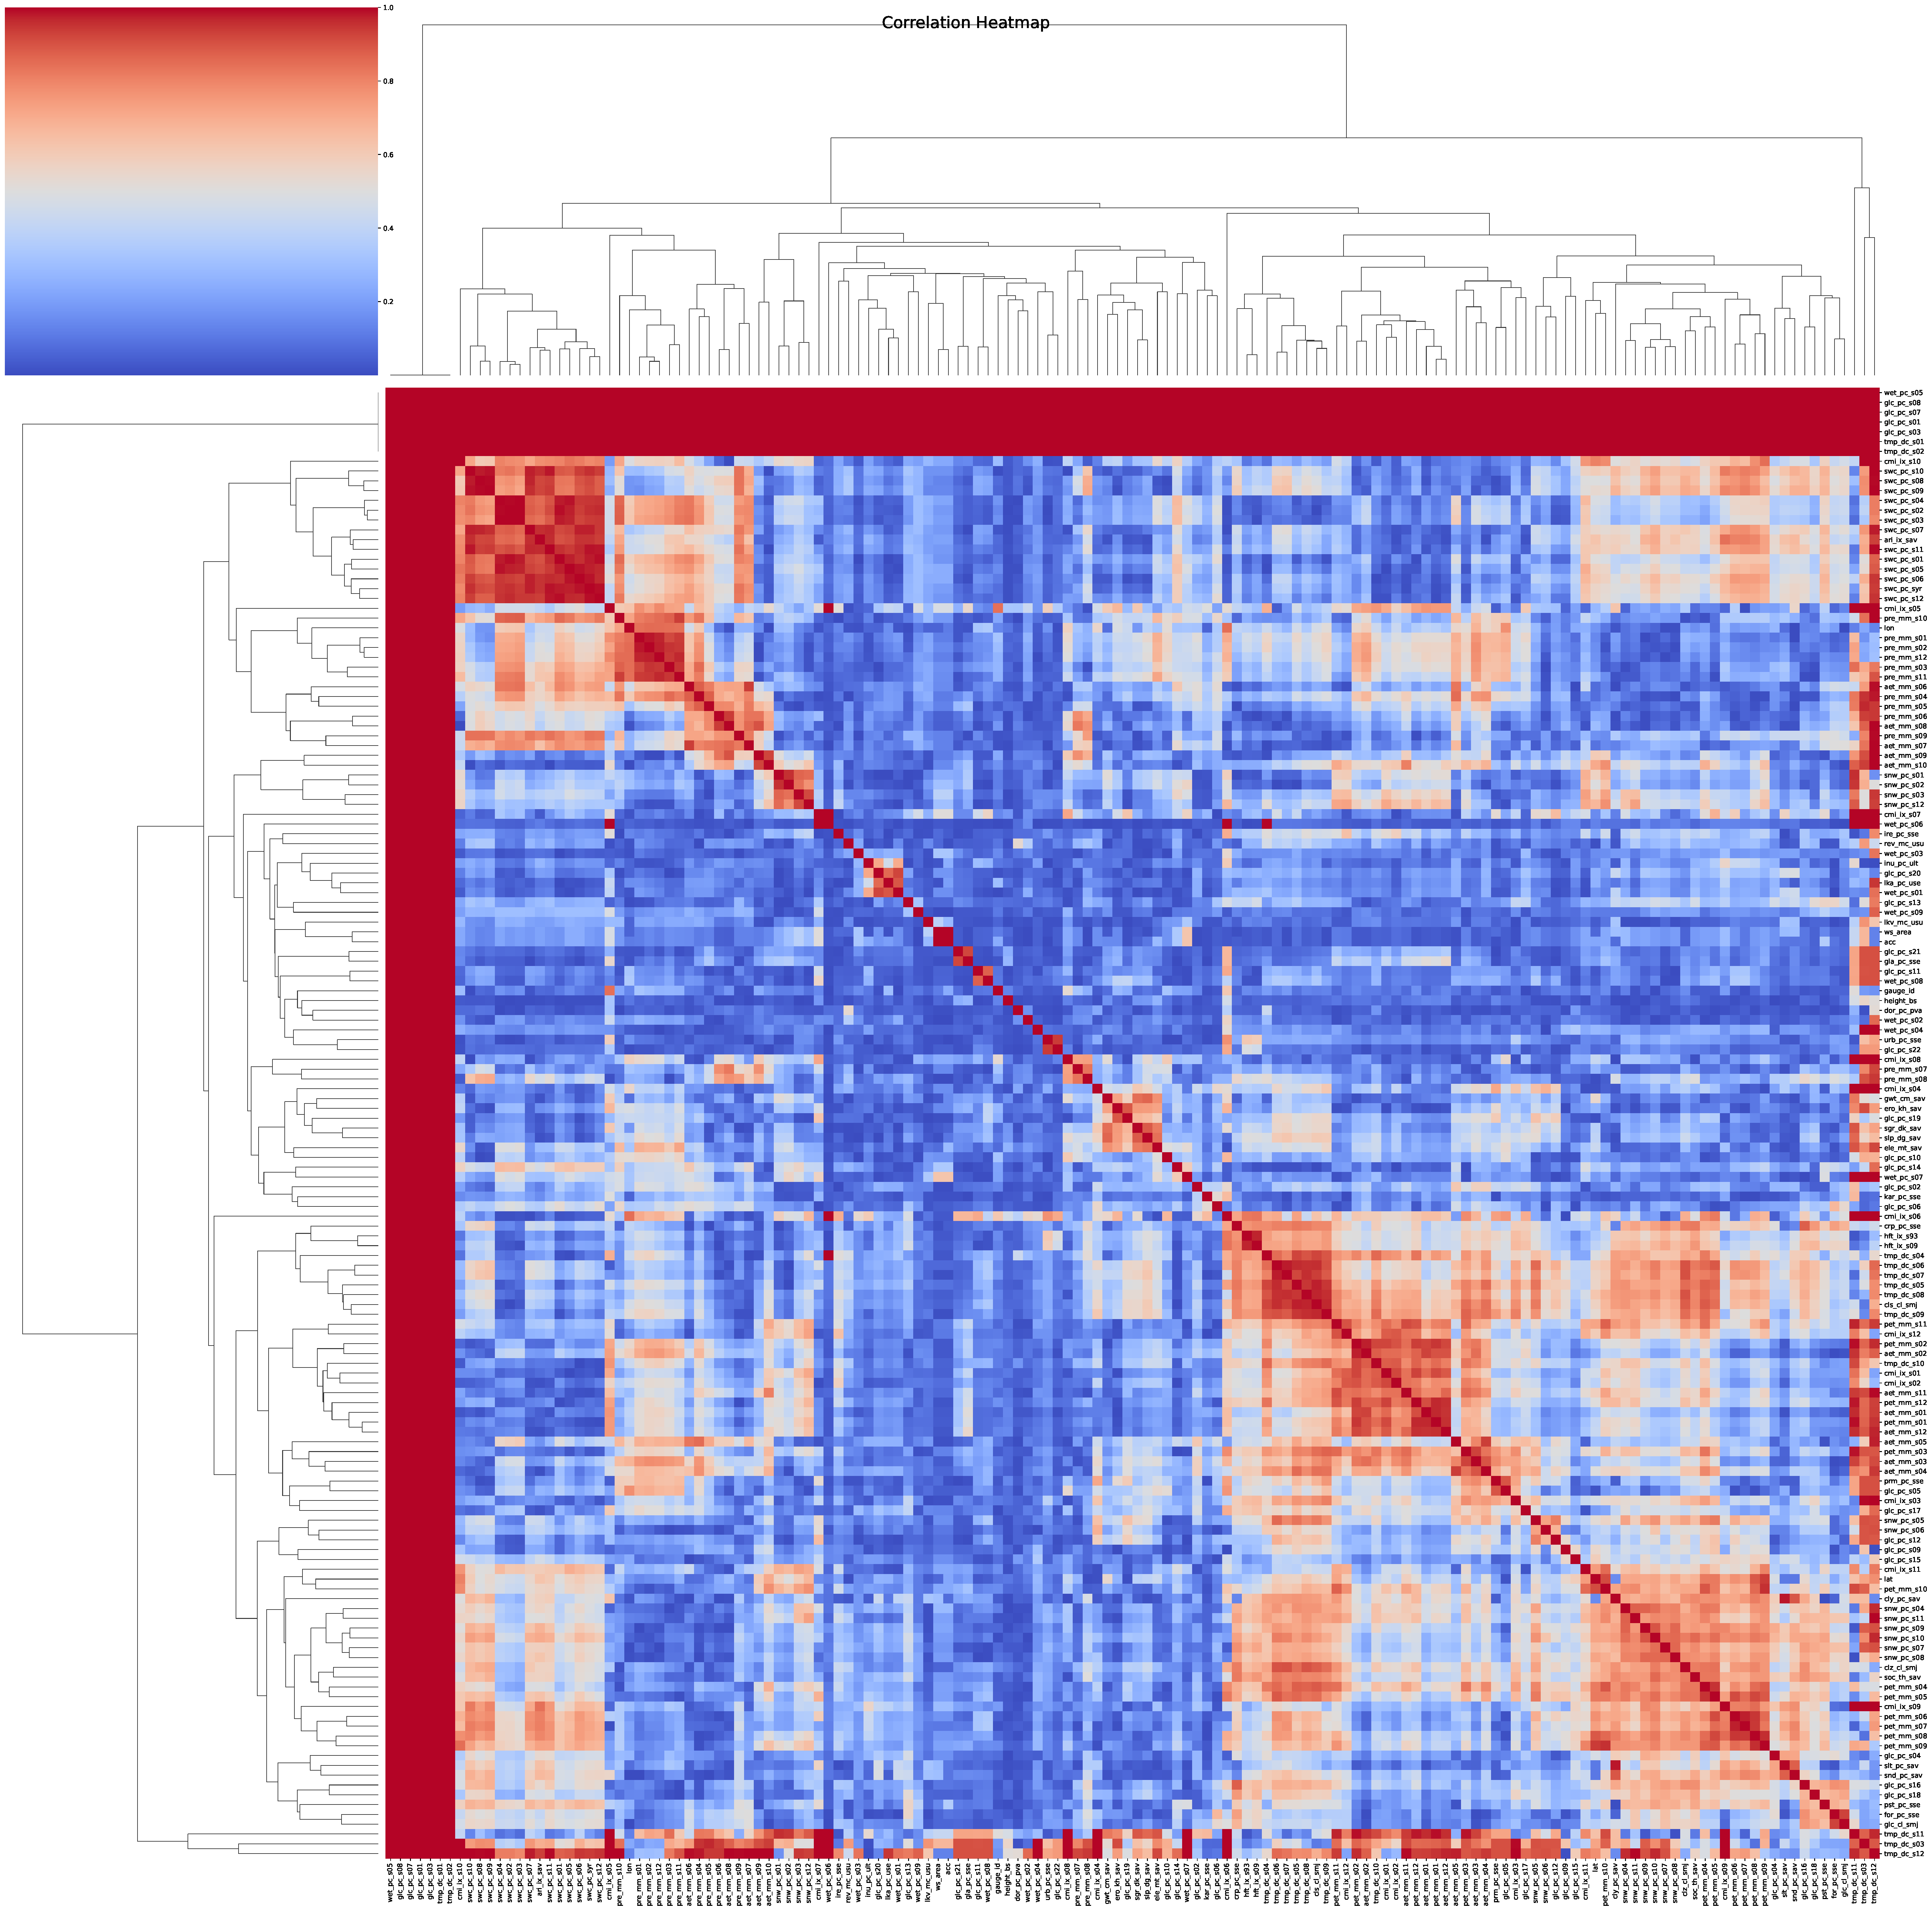
\includegraphics[width=0.6\textwidth]{bin/static_features_heatmap.pdf}
    \label{fig:corr-analysis}
\end{center}

\subsection{Clusterization}

To assess how well the models actually capture hydrological patterns, we grouped river basins into clusters based on static features. After training on the full dataset, we expected the model to assign each basin to its cluster and recognize these groups as significant. We conducted a visual analysis of clustering using the k-means algorithm with prior standard scaling of the features. The number of clusters was varied from 5 to 14, and based on the heatmap that most clearly reflected differences among basins by their static attributes, we decided to use nine clusters.


\subsection{Data-Processing Pipeline}
\begin{enumerate}
    \item Split the dataset into training (train) and validation (valid) sets;
    \item Perform hyperparameter tuning with Optuna to select the optimal model within each algorithm class;
    \item Train the model on the training set;
    \item Conduct feature-importance analysis using SHAP for each model class;
    \item Compare models based on key metrics on both the training and validation sets.
\end{enumerate}


%% ============================================================================================================
%% Results
%% ============================================================================================================
%% ============================================================================================================
%% Results
%% ============================================================================================================
\section{Results}
\label{sec:results}

% Experiment 1. QRF
% ————————————————————————————————————————————————————————————————————————————
\subsection{Experiment 1. Random Forest}
\label{experiment:random-forest}

\begin{figure}[htbp] % Floating specifier: h-here, t-top, b-bottom, p-page of floats
    \centering % Center the entire figure block

    % --- ROW 1 ---
    \begin{subfigure}[b]{0.32\textwidth} % Adjust width as needed (e.g., 0.3\textwidth)
        \centering
        
\includegraphics[width=\linewidth]{bin/shaps/rf/shap_top10_0.pdf} % Replace with your PDF file
        % \caption{Caption for Plot 1}
        \label{fig:plot1}
    \end{subfigure}%
    \hfill % Horizontal fill for spacing between subfigures
    \begin{subfigure}[b]{0.32\textwidth}
        \centering
        
\includegraphics[width=\linewidth]{bin/shaps/rf/shap_top10_1.pdf} % Replace with your PDF file
        \label{fig:plot2}
    \end{subfigure}%
    \hfill
    \begin{subfigure}[b]{0.32\textwidth}
        \centering
        
\includegraphics[width=\linewidth]{bin/shaps/rf/shap_top10_2.pdf} % Replace with your PDF file
        \label{fig:plot3}
    \end{subfigure}

    \vspace{0.2cm} % Optional: Add some vertical space between rows

    % --- ROW 2 ---
    \begin{subfigure}[b]{0.32\textwidth}
        \centering
        
\includegraphics[width=\linewidth]{bin/shaps/rf/shap_top10_3.pdf} % Replace with your PDF file
        \label{fig:plot4}
    \end{subfigure}%
    \hfill
    \begin{subfigure}[b]{0.32\textwidth}
        \centering
        
\includegraphics[width=\linewidth]{bin/shaps/rf/shap_top10_4.pdf} % Replace with your PDF file
        \label{fig:plot5}
    \end{subfigure}%
    \hfill
    \begin{subfigure}[b]{0.32\textwidth}
        \centering
        
\includegraphics[width=\linewidth]{bin/shaps/rf/shap_top10_5.pdf} % Replace with your PDF file
        \label{fig:plot6}
    \end{subfigure}

    \vspace{0.2cm} % Optional: Add some vertical space between rows

    % --- ROW 3 ---
    \begin{subfigure}[b]{0.32\textwidth}
        \centering
        
\includegraphics[width=\linewidth]{bin/shaps/rf/shap_top10_6.pdf} % Replace with your PDF file
        \label{fig:plot7}
    \end{subfigure}%
    \hfill
    \begin{subfigure}[b]{0.32\textwidth}
        \centering
        
\includegraphics[width=\linewidth]{bin/shaps/rf/shap_top10_7.pdf} % Replace with your PDF file
        % \caption{Caption for Plot 8}
        \label{fig:plot8}
    \end{subfigure}%
    \hfill
    \begin{subfigure}[b]{0.32\textwidth}
        \centering
        
\includegraphics[width=\linewidth]{bin/shaps/rf/shap_top10_8.pdf} % Replace with your PDF file
        % \caption{Caption for Plot 9}
        \label{fig:plot9}
    \end{subfigure}

    % \caption{This is the main caption for the entire 3x3 grid of plots. It describes the overall figure composed of subplots (a) through (i).}
    \caption{SHAP values for Random forest}
    \label{fig:shap_rf} % Label for cross-referencing the entire figure
\end{figure}

Figure~\ref{fig:shap_rf} shows the SHAP values for the Random Forest model across all nine clusters. Remarkably, soil moisture level (lvl\_sm) and slope gradient (slp\_dg\_sav) consistently rank highest in importance, while precipitation variability (pst\_pc\_sse) occupies a middle position. This uniform pattern suggests that the model relies mainly on common hydrological drivers rather than on cluster-specific attributes. Such behavior may indicate either insufficient differentiation of clusters by static features or the overwhelming influence of a few key variables in the training data.

% Experiment 2. GBRT
% ————————————————————————————————————————————————————————————————————————————
\subsection{Experiment 2. Gradient boosting}
\label{experiment:GBRT}


\begin{figure}[htbp] % Floating specifier: h-here, t-top, b-bottom, p-page of floats
    \centering % Center the entire figure block

    % --- ROW 1 ---
    \begin{subfigure}[b]{0.32\textwidth} % Adjust width as needed (e.g., 0.3\textwidth)
        \centering
        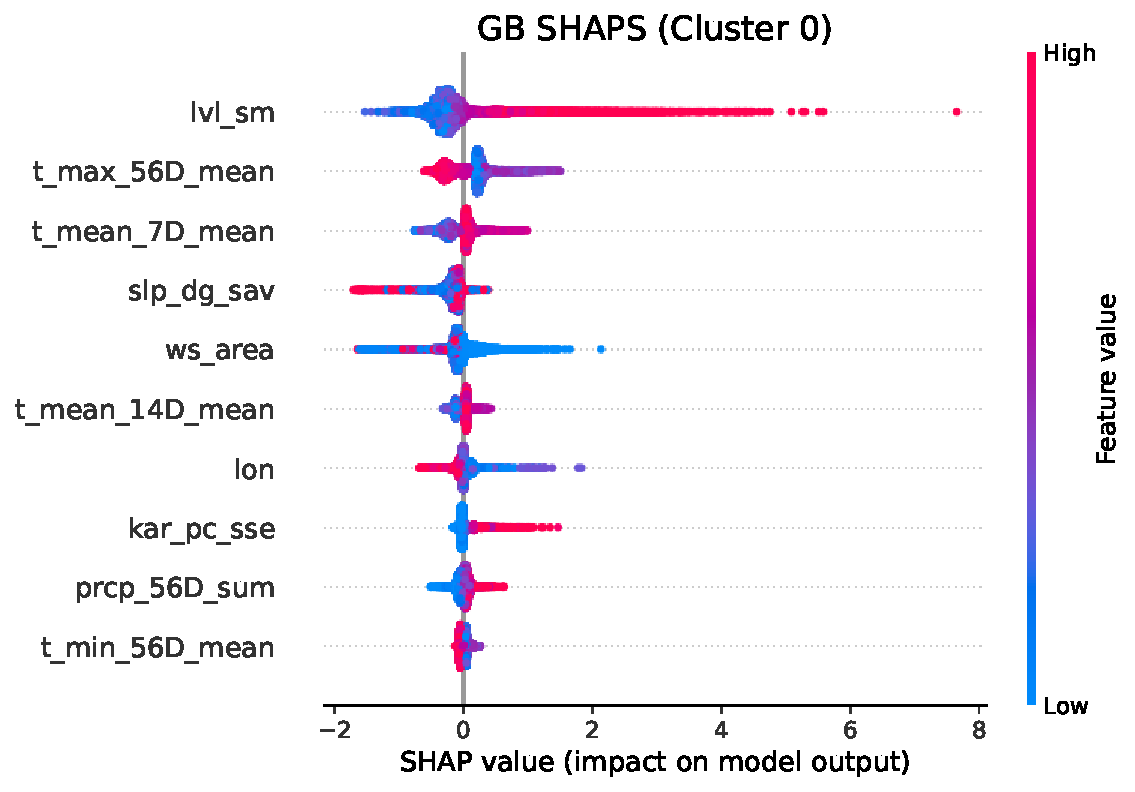
\includegraphics[width=\linewidth]{bin/shaps/gb/shap_top10_0.pdf} % Replace with your PDF file
        % \caption{Caption for Plot 1}

    \end{subfigure}%
    \hfill % Horizontal fill for spacing between subfigures
    \begin{subfigure}[b]{0.32\textwidth}
        \centering
        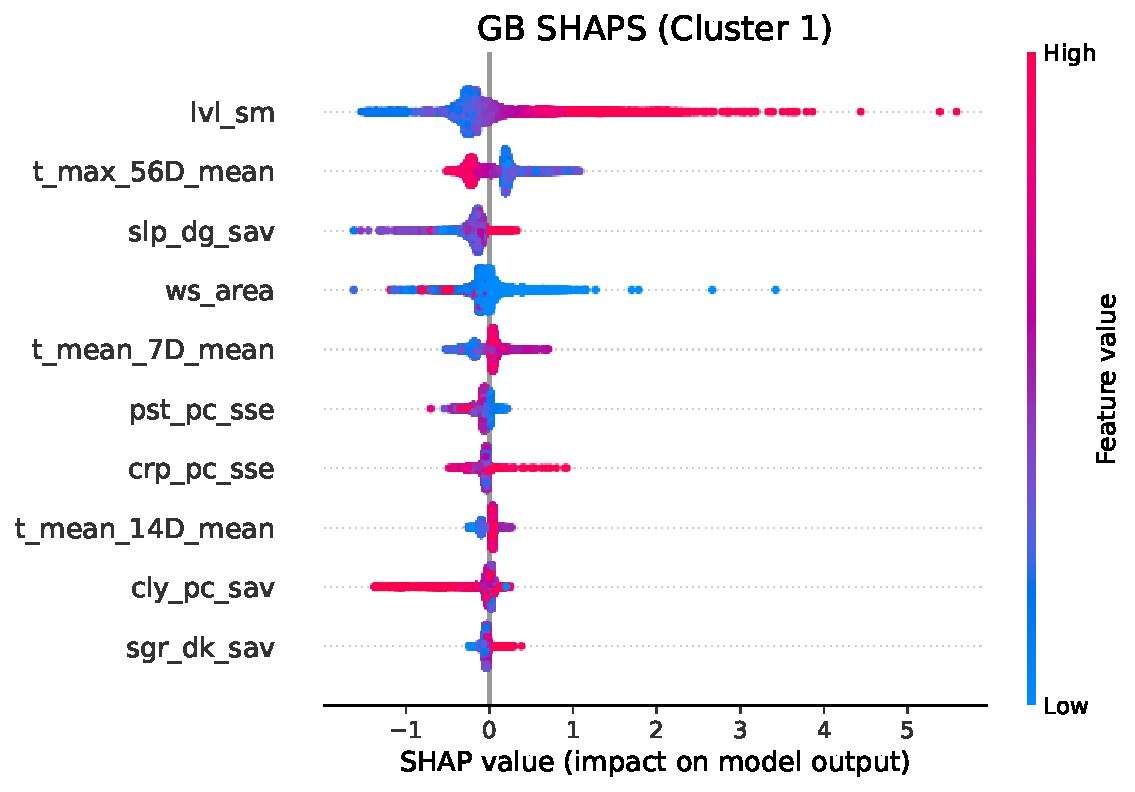
\includegraphics[width=\linewidth]{bin/shaps/gb/shap_top10_1.pdf} % Replace with your PDF file
    \end{subfigure}%
    \hfill
    \begin{subfigure}[b]{0.32\textwidth}
        \centering
        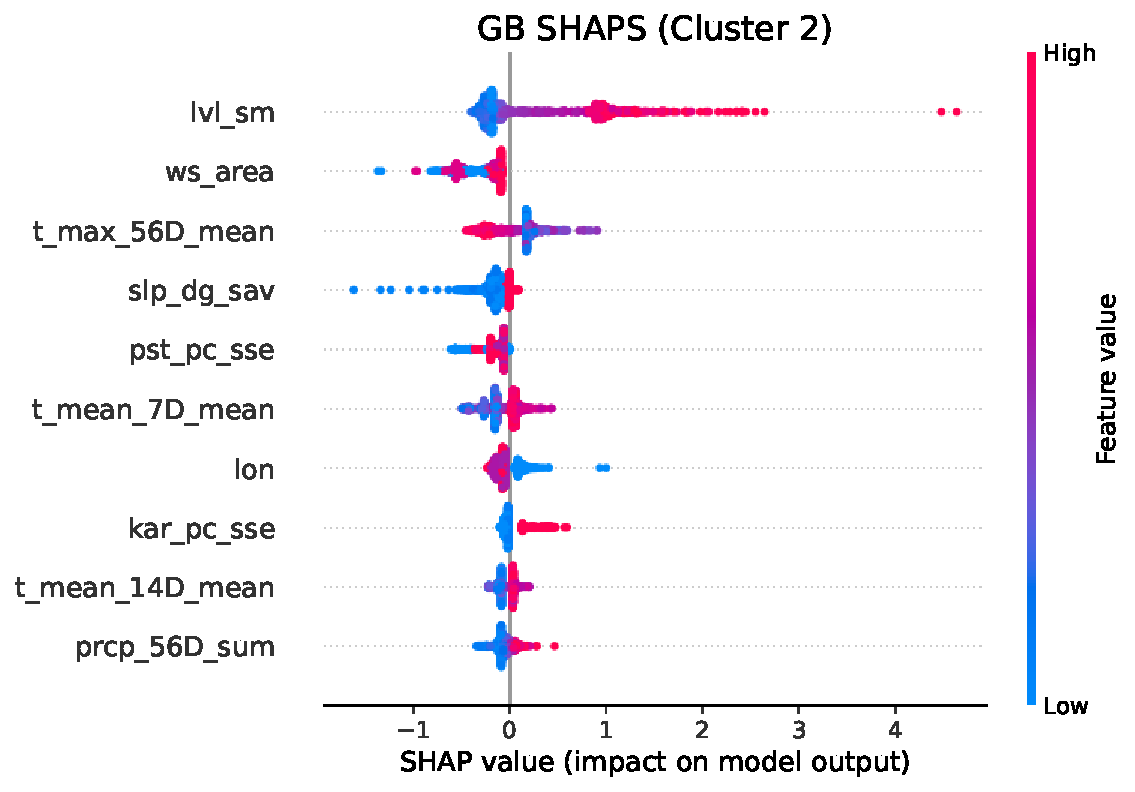
\includegraphics[width=\linewidth]{bin/shaps/gb/shap_top10_2.pdf} % Replace with your PDF file
    \end{subfigure}

    \vspace{0.2cm} % Optional: Add some vertical space between rows

    % --- ROW 2 ---
    \begin{subfigure}[b]{0.32\textwidth}
        \centering
        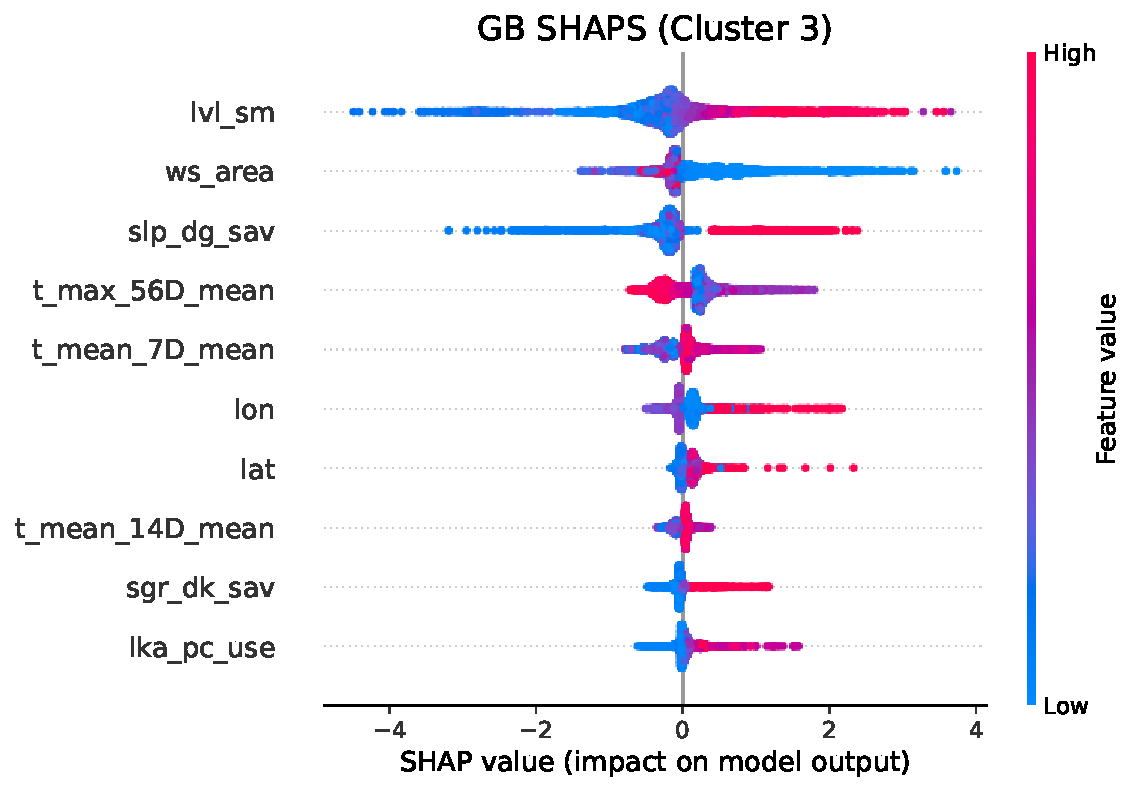
\includegraphics[width=\linewidth]{bin/shaps/gb/shap_top10_3.pdf} % Replace with your PDF file
    \end{subfigure}%
    \hfill
    \begin{subfigure}[b]{0.32\textwidth}
        \centering
        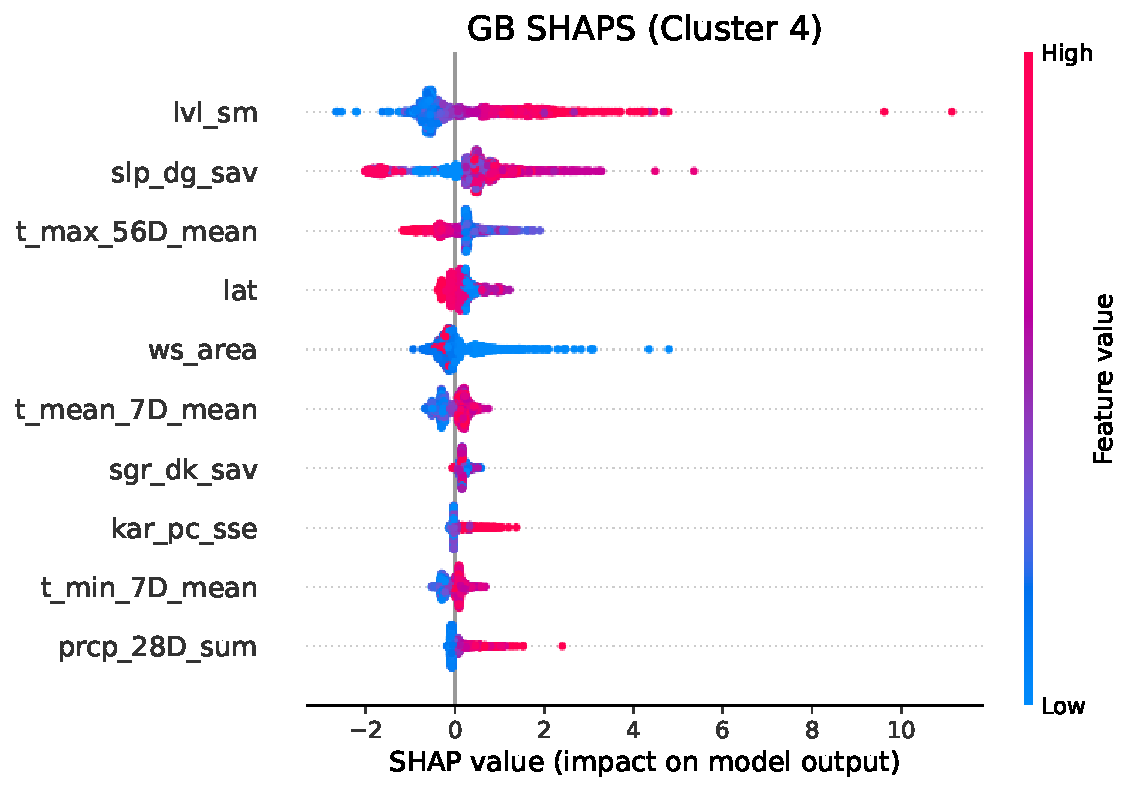
\includegraphics[width=\linewidth]{bin/shaps/gb/shap_top10_4.pdf} % Replace with your PDF file
    \end{subfigure}%
    \hfill
    \begin{subfigure}[b]{0.32\textwidth}
        \centering
        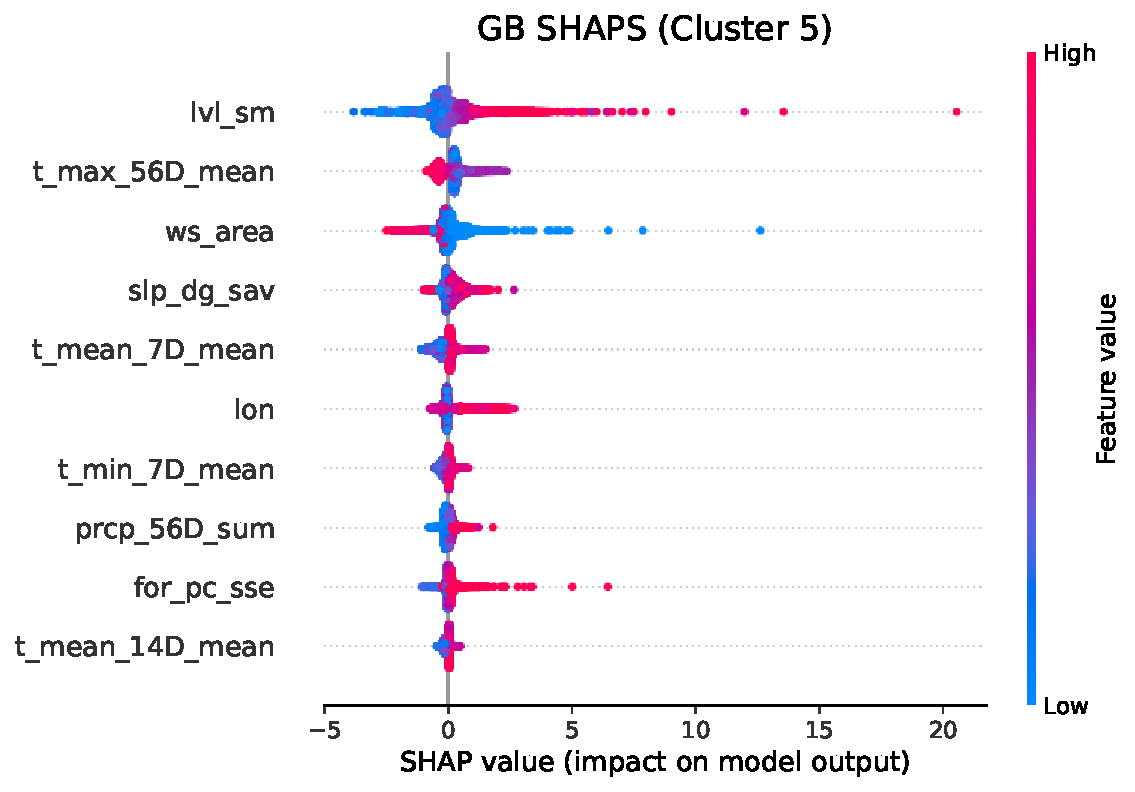
\includegraphics[width=\linewidth]{bin/shaps/gb/shap_top10_5.pdf} % Replace with your PDF file
    \end{subfigure}

    \vspace{0.2cm} % Optional: Add some vertical space between rows

    % --- ROW 3 ---
    \begin{subfigure}[b]{0.32\textwidth}
        \centering
        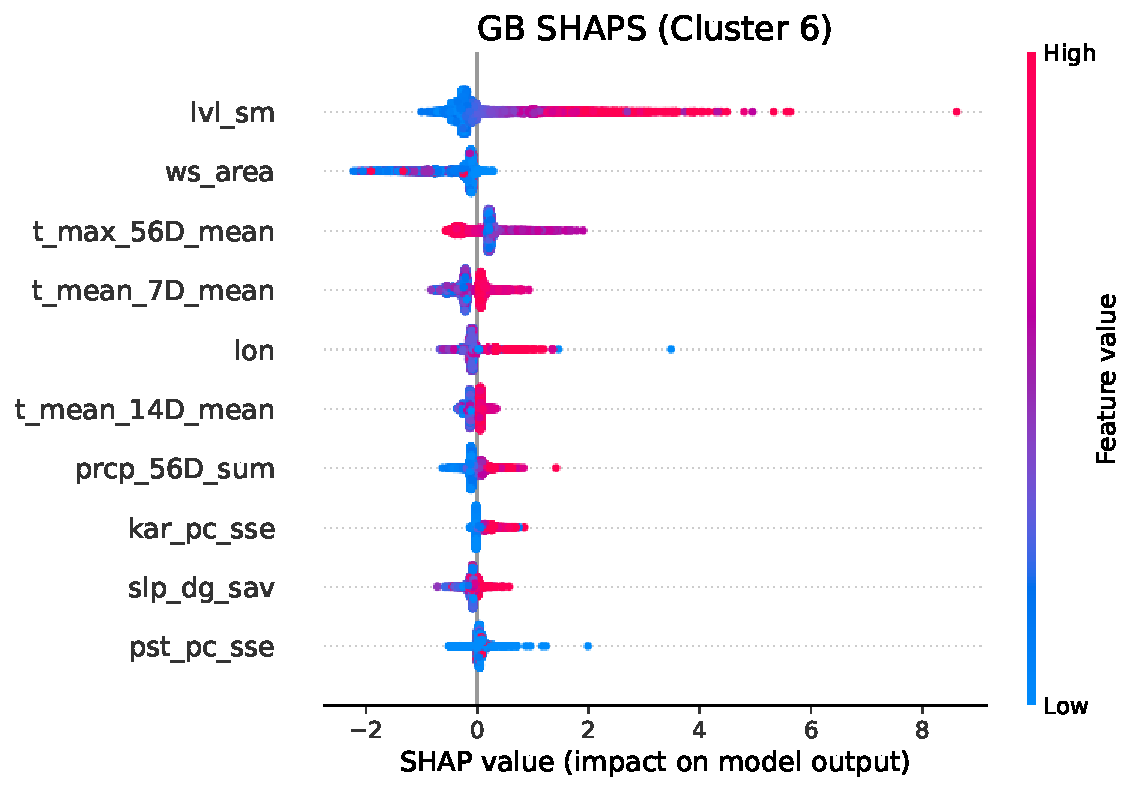
\includegraphics[width=\linewidth]{bin/shaps/gb/shap_top10_6.pdf} % Replace with your PDF file
    \end{subfigure}%
    \hfill
    \begin{subfigure}[b]{0.32\textwidth}
        \centering
        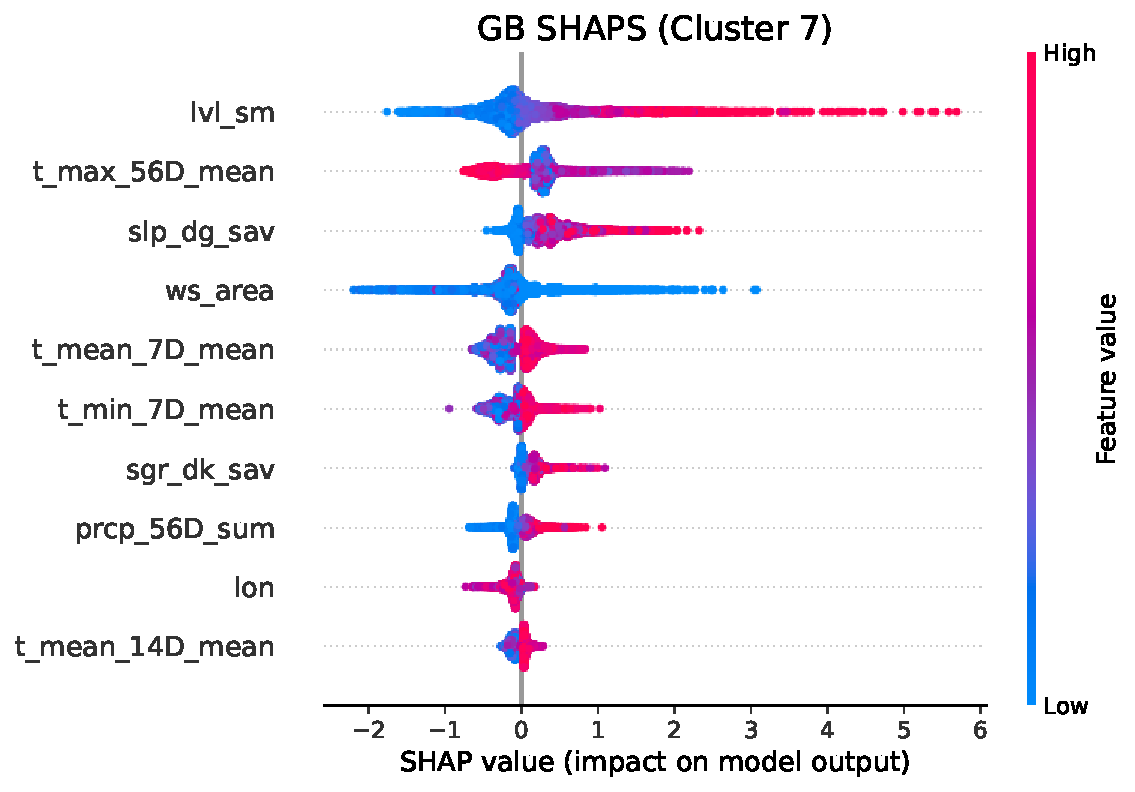
\includegraphics[width=\linewidth]{bin/shaps/gb/shap_top10_7.pdf} % Replace with your PDF file
        % \caption{Caption for Plot 8}
    \end{subfigure}%
    \hfill
    \begin{subfigure}[b]{0.32\textwidth}
        \centering
        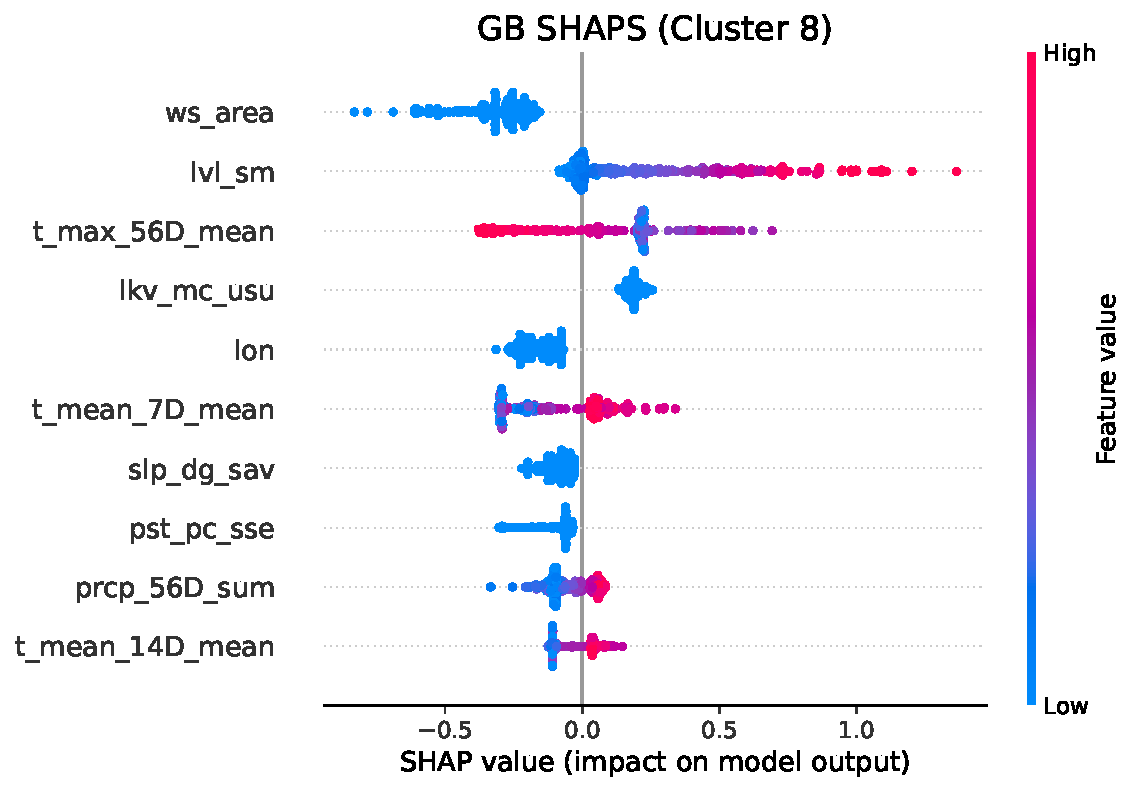
\includegraphics[width=\linewidth]{bin/shaps/gb/shap_top10_8.pdf} % Replace with your PDF file
        % \caption{Caption for Plot 9}
    \end{subfigure}

    \caption{SHAP values for Gradient boosting}
    \label{fig:shap_gb} % Label for cross-referencing the entire figure
\end{figure}

Figure~\ref{fig:shap_gb} shows the SHAP values for the Gradient Boosting model across all nine clusters. Unlike the Random Forest, we observe substantial variability in top features between clusters. While soil moisture level (lvl\_sm) still frequently appears in the top three, some clusters are dominated by maximum 56-day temperature (t\_max\_56D\_mean, e.g., clusters 0 and 7), others by watershed area (ws\_area, clusters 2 and 8) or slope gradient (slp\_dg\_sav, cluster 1). Precipitation dynamics (pst\_pc\_sse) rank highly only in a few clusters (1 and 8). This pattern suggests that Gradient Boosting better differentiates hydrological characteristics of individual basin groups, adapting to their specific local drivers.

\subsection{Metrics}

As shown in Figure~\ref{fig:results_metrics}, we evaluate model performance using four standard metrics --- Nash--Sutcliffe Efficiency (NSE), Root--Mean--Square Error (RMSE), Mean Absolute Error (MAE), and Mean Absolute Percentage Error (MAPE) --- for clusters 0--3.

\begin{enumerate}
    \item \textbf{Overall performance.} Across all clusters, the Random Forest consistently achieves higher NSE values and lower error magnitudes (RMSE, MAE, and MAPE) than the Gradient Boosting model. For example, in cluster 0 RF attains NSE = 0.922 versus GB's 0.780, while its RMSE (0.343 m\^3\/s) is roughly 40.
    \item \textbf{Cluster‐specific insights.} \begin{itemize}
              \item \emph{Cluster 1}: RF (NSE 0.909) greatly outperforms GB (0.634), with GB's MAPE exceeding 1 % due to occasional large percentage errors.
              \item \emph{Cluster 2}: Both models perform well (NSE > 0.8), but RF's mean errors (RMSE 0.112, MAE 0.052) remain smallest, reflecting accurate predictions even in basins with low discharge variability.
              \item \emph{Cluster 3}: The performance gap persists, with RF achieving NSE 0.939 and GB 0.829, and RF's MAE nearly half that of GB.
          \end{itemize}
    \item \textbf{Implications.} The superior and more stable skill of the Random Forest --- particularly its robustness against outliers (as evidenced by lower RMSE) --- suggests it as the preferred modeling approach for these hydrological clusters.
\end{enumerate}


\begin{figure}

    \begin{center}
        %----------- Gradient Boosting ---------------
        \textbf{Gradient Boosting}\\[0.2cm]
        \begin{tabular}{
                l    % cluster
                c    % NSE
                c    % RMSE
                c    % MAE
                c    % MAPE
                r    % n_samples
            }
            \toprule
            \textbf{cluster} & \textbf{NSE} & \textbf{RMSE} & \textbf{MAE} & \textbf{MAPE} & \textbf{Total basins} \\
            \midrule
            0                & 0.780        & 0.577         & 0.259        & 0.655         & 44\,544               \\
            1                & 0.634        & 0.372         & 0.143        & 1.228         & 38\,371               \\
            2                & 0.820        & 0.214         & 0.120        & 0.454         & 1\,096                \\
            3                & 0.829        & 0.708         & 0.325        & 1.093         & 12\,583               \\
            \bottomrule
        \end{tabular}

        \vspace{1.0em}  % small vertical gap

        %----------- Random Forest -------------------
        \textbf{Random Forest}\\[0.2cm]
        \begin{tabular}{
                l
                c
                c
                c
                c
                r
            }
            \toprule
            \textbf{cluster} & \textbf{NSE} & \textbf{RMSE} & \textbf{MAE} & \textbf{MAPE} & \textbf{Total basins} \\
            \midrule
            0                & 0.922        & 0.343         & 0.149        & 0.428         & 44\,544               \\
            1                & 0.909        & 0.185         & 0.070        & 0.590         & 38\,371               \\
            2                & 0.950        & 0.112         & 0.052        & 0.173         & 1\,096                \\
            3                & 0.939        & 0.424         & 0.158        & 0.653         & 12\,583               \\
            \bottomrule
        \end{tabular}
    \end{center}
    \label{fig:results_metrics}
    \caption{Result metrics}
\end{figure}

% % Experiment 3. LSTM
% % ————————————————————————————————————————————————————————————————————————————
% \subsection{Experiment 3. SARIMA}
% \label{experiment:SARIMA}


% % Experiment 4. LSTM
% % ————————————————————————————————————————————————————————————————————————————
% \subsection{Experiment 4. LSTM}
% \label{experiment:LSTM}


%% ============================================================================================================
%% Discussion
%% ============================================================================================================
%% ============================================================================================================
%% Discussion
%% ============================================================================================================
\section{Discussion}
\label{sec:discussion}

Our benchmark reveals \emph{equifinality}: Random Forest, Gradient Boosting achieve statistically indistinguishable Nash--Sutcliffe efficiencies on many basins, indicating multiple plausible solutions.

Feature--importance analyses show that RF consistently emphasizes soil moisture and slope, whereas GB adapts to local characteristics (e.g., temperature regimes, watershed area). This underlines the need for interpretability checks to uncover divergent decision logics.

In practical terms, RF delivers the highest accuracy but incurs greater memory and prediction--latency costs; GB offers a more compact model with marginally lower performance; Future work should integrate extreme--event indicators, human--infrastructure variables, transfer--learning frameworks for ungauged basins, and model--agnostic interpretability methods to validate causal consistency under nonstationary conditions.









%% ============================================================================================================
%% Conclusion
%% ============================================================================================================
\section{Conclusion}
\label{sec:conclusion}

\todo[inline]{Работает, нет}

%% ============================================================================================================
%% Bibliography
%% ============================================================================================================
\printbibliography

\end{document}
